\documentclass{article}
\usepackage{amsmath}
\usepackage{graphicx}
\usepackage{hyperref}
\usepackage{float}

\title{PHYS11 CH3}
\author{Mr. Gullo}
\date{September 2024}

\begin{document}

\maketitle

\section{Introduction}

In physics, understanding motion is crucial for analyzing how objects move in space and time. One of the fundamental concepts is \textbf{acceleration}, which describes how an object's velocity changes over time. This lesson covers the essential skills and concepts needed to solve problems involving acceleration, including average acceleration, kinematic equations, graphical analysis, and vector directions.

\section{Acceleration}

\subsection{Definition of Acceleration}

Acceleration is defined as the rate at which an object's velocity changes with time. It is a vector quantity, meaning it has both magnitude and direction.

\begin{equation}
\vec{a} = \frac{\Delta \vec{v}}{\Delta t}
\end{equation}

where:
\begin{itemize}
    \item \( \vec{a} \) is the acceleration,
    \item \( \Delta \vec{v} = \vec{v} - \vec{v}_0 \) is the change in velocity,
    \item \( \Delta t = t - t_0 \) is the change in time.
\end{itemize}

\subsection{Average Acceleration}

Average acceleration over a time interval is calculated by dividing the change in velocity by the time over which the change occurs.

\begin{equation}
\vec{a}_{\text{avg}} = \frac{\vec{v} - \vec{v}_0}{t - t_0}
\end{equation}

\section{Kinematic Equations for Uniform Acceleration}

When acceleration is constant, the motion of an object can be described using the following kinematic equations:

\begin{align}
\vec{v} &= \vec{v}_0 + \vec{a}t \label{eq1} \\
\vec{x} &= \vec{x}_0 + \vec{v}_0 t + \tfrac{1}{2} \vec{a} t^2 \label{eq2} \\
v^2 &= v_0^2 + 2a (x - x_0) \label{eq3}
\end{align}

where:
\begin{itemize}
    \item \( \vec{v} \) is the final velocity,
    \item \( \vec{v}_0 \) is the initial velocity,
    \item \( \vec{a} \) is the acceleration,
    \item \( t \) is the time,
    \item \( \vec{x} \) is the final position,
    \item \( \vec{x}_0 \) is the initial position.
\end{itemize}

\section{Graphical Analysis}

\subsection{Velocity vs. Time Graphs}

In a velocity vs. time graph:
\begin{itemize}
    \item The \textbf{slope} of the line represents acceleration.
    \item A \textbf{straight line} indicates constant acceleration.
    \item A \textbf{curved line} indicates changing acceleration.
\end{itemize}

\subsection{Displacement vs. Time Graphs}

In a displacement vs. time graph:
\begin{itemize}
    \item The \textbf{slope} of the line represents velocity.
    \item A \textbf{straight line} indicates constant velocity (zero acceleration).
    \item A \textbf{curved line} indicates changing velocity (non-zero acceleration).
\end{itemize}

\section{Vectors and Direction}

Acceleration, velocity, and displacement are vector quantities. The direction of these vectors is significant:

\begin{itemize}
    \item \textbf{Positive acceleration} means the acceleration vector points in the positive direction.
    \item \textbf{Negative acceleration} (deceleration) means the acceleration vector points in the negative direction.
    \item Positive and negative vectors point in opposite directions (180° apart).
\end{itemize}
\newpage
\section{Worked Examples}

\subsection{Example 1: Calculating Average Acceleration}

\textbf{Problem:} If a velocity increases from 0 to 20 m/s in 10 s, what is the average acceleration?

\textbf{Solution:}

Given:
\begin{align*}
\vec{v}_0 &= 0 \, \text{m/s} \\
\vec{v} &= 20 \, \text{m/s} \\
t &= 10 \, \text{s}
\end{align*}

Using the average acceleration formula:
\begin{align*}
\vec{a}_{\text{avg}} &= \frac{\vec{v} - \vec{v}_0}{t} \\
&= \frac{20 \, \text{m/s} - 0 \, \text{m/s}}{10 \, \text{s}} \\
&= \frac{20 \, \text{m/s}}{10 \, \text{s}} \\
&= 2 \, \text{m/s}^2
\end{align*}

\textbf{Answer:} The average acceleration is \( 2 \, \text{m/s}^2 \).
\newpage
\subsection{Example 2: Interpreting Velocity vs. Time Graphs}

\textbf{Problem:} The image shows a velocity vs. time graph for a jet car. Show that, if you take the slope at any point on the graph, the jet car's acceleration will be \( 5.0 \, \text{m/s}^2 \).


\begin{figure}[H]
    \centering
    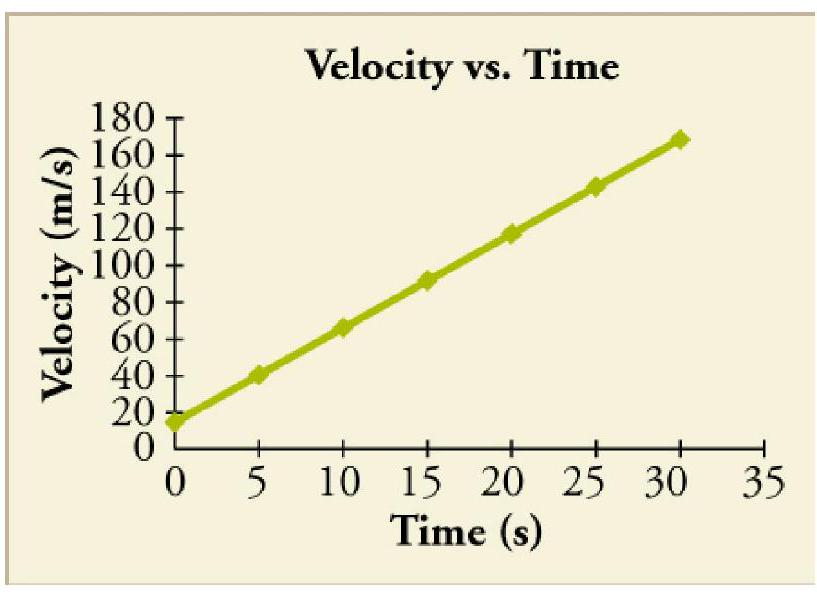
\includegraphics[width=0.75\linewidth]{2024_09_22_d75bb9ada91612339d1ag-12.jpg}
\caption{Velocity vs. Time Graph for a Jet Car}
\end{figure}



\textbf{Solution:}

On a velocity vs. time graph:
\begin{itemize}
    \item The slope of the line (\( \frac{\Delta \vec{v}}{\Delta t} \)) represents acceleration.
    \item If the line is straight, the acceleration is constant.
\end{itemize}

Calculating the slope:
\begin{align*}
\text{Slope} &= \frac{\Delta \vec{v}}{\Delta t} \\
&= \frac{\vec{v}_2 - \vec{v}_1}{t_2 - t_1}
\end{align*}

From the graph (assuming the line goes from \( (0, 0) \) to \( (t, v) \)):
\begin{align*}
\text{Slope} &= \frac{\vec{v}}{t}
\end{align*}

Given that the slope is constant and equal to \( 5.0 \, \text{m/s}^2 \) throughout the graph.

\textbf{Answer:} True. The acceleration is \( 5.0 \, \text{m/s}^2 \) at any point on the graph.
\newpage
\subsection{Example 3: Calculating Total Time with Acceleration and Deceleration}

\textbf{Problem:} A car accelerates from rest at a stop sign at a rate of \( 3.0 \, \text{m/s}^2 \) to a speed of \( 21.0 \, \text{m/s} \), and then immediately begins to decelerate to a stop at the next stop sign at a rate of \( 4.0 \, \text{m/s}^2 \). How long did it take the car to travel from the first stop sign to the second stop sign?

\textbf{Solution:}

\underline{First Phase (Acceleration):}

Given:
\begin{align*}
\vec{v}_0 &= 0 \, \text{m/s} \\
\vec{v} &= 21.0 \, \text{m/s} \\
\vec{a} &= 3.0 \, \text{m/s}^2
\end{align*}

Using Equation \eqref{eq1}:
\begin{align*}
t_1 &= \frac{\vec{v} - \vec{v}_0}{\vec{a}} \\
&= \frac{21.0 \, \text{m/s} - 0 \, \text{m/s}}{3.0 \, \text{m/s}^2} \\
&= 7.0 \, \text{s}
\end{align*}

\underline{Second Phase (Deceleration):}

Given:
\begin{align*}
\vec{v}_0 &= 21.0 \, \text{m/s} \\
\vec{v} &= 0 \, \text{m/s} \\
\vec{a} &= -4.0 \, \text{m/s}^2 \quad (\text{negative since it's deceleration})
\end{align*}

Using Equation \eqref{eq1}:
\begin{align*}
t_2 &= \frac{\vec{v} - \vec{v}_0}{\vec{a}} \\
&= \frac{0 \, \text{m/s} - 21.0 \, \text{m/s}}{ -4.0 \, \text{m/s}^2} \\
&= \frac{-21.0 \, \text{m/s}}{ -4.0 \, \text{m/s}^2} \\
&= 5.25 \, \text{s}
\end{align*}

\textbf{Total Time:}
\begin{align*}
t_{\text{total}} &= t_1 + t_2 \\
&= 7.0 \, \text{s} + 5.25 \, \text{s} \\
&= 12.25 \, \text{s}
\end{align*}

However, since the options provided in the original problem do not include \( 12.25 \, \text{s} \), and the closest value is \( 12 \, \text{s} \), we can conclude that the total time is approximately \( 12 \, \text{s} \).

\textbf{Answer:} It took the car approximately \( 12 \, \text{s} \) to travel between the stop signs.

\section{Conclusion}

Understanding acceleration and the equations of motion for uniformly accelerated objects is essential in physics. By mastering these concepts, you can analyze various real-world situations, such as calculating the time it takes for a car to travel between two points or interpreting motion graphs accurately.

\end{document}